\clearpage
\subsection{Results from "ibmt43" [df6407d], generated Sun Sep 25 23:16:47 CEST 2011}
\begin{verbatim}

Test aspects:

    compilation:
        compilation time measured by 'time' call
        only 'real' time is taken into account
        result is in seconds

    size:
        size of the binary measured by 'ls -k' call
        result is in kilobytes

    strip-size:
        size of the binary measured by 'ls -k' call after 'strip' call
        result is in kilobytes

    execution:
        execution time measured by 'time' call
        only 'real' time is taken into account
        result is in seconds

    valgrind:
        test is executed with valgrind call
        result is as A/D (S), where
        A - allocations
        D - deallocations
        S - global allocated size in bytes

    test name:
        test_NAME[_NUMBER], where NAME is test case name and NUMBER is count of event calls during the test
\end{verbatim}
\begin{center}
\line(1,0){750}
\end{center}
\begin{verbatim}

Environment statistics:

    generated: Sun Sep 25 23:16:47 CEST 2011
    code revision: df6407d
    hostname: "ibmt43"
    operating system:  GNU/Linux
    processor: Intel(R) Pentium(R) M processor 1.86GHz
    free memory: 495Mb
    load average: 0.97 0.97 0.87 2/108 14066
\end{verbatim}
\begin{center}
\line(1,0){750}
\end{center}
\begin{verbatim}

All tests summary:

    real: 1643.09s (27:23.09)
    user: 1578.01s
    sys: 16.30s
    cpu: 97%
    average memory usage: 0K
    maximum resident set size: 0K
    number of times the process was swapped out of main memory: 0
    number of file system input: 0
    number of file system outputs: 0
\end{verbatim}
\begin{center}
\line(1,0){750}
\end{center}
\begin{verbatim}
Results are presented by using table and two types of charts:

    table: contains results for each tested aspect and framework
    first type of chart: presents relative (0-100%) differents between individual framework and aspect
    second type of chart: presents each aspect individually using exact values returned during the test
\end{verbatim}
\begin{center}
\line(1,0){750}
\end{center}
\begin{landscape}
\begin{table}
\caption{"ibmt43" [df6407d], g++-4.3.2 -m32/test transitions 1000000}
\centering
\begin{longtable}{| c | c |c |c |c |c |c |c |}
\hline
& CFsmBase& StateChart& MSM.favor\_runtime\_speed& MSM.favor\_compile\_time& QFsm.FavorExecutionSpeed& QFsm.FavorCompilationTime& QFsm.FavorDebugSize\\
\hline
compilation & 0.89s & 1.24s & 3.15s & 3.10s & 0.88s & 0.82s & 0.91s\\
\hline
size & 38K & 113K & 104K & 122K & 27K & 20K & 40K\\
\hline
strip-size & 22K & 46K & 34K & 38K & 10K & 10K & 18K\\
\hline
execution & 0.08s & 1.49s & 0.46s & 0.60s & 0.10s & 0.21s & 0.34s\\
\hline
valgrind & 9/9 (138b) & 1,000,004/1,000,004 (24,000,064b) & 4/4 (561b) & 10/10 (2,673b) & 2/2 (17b) & 2/2 (17b) & 16/16 (241b)\\
\hline
\multicolumn{8}{|c|}{\includegraphics[scale=0.8]{images/"results/ibmt43"/"g++-4.3.2 -m32"/test_transitions_1000000_all.png}}\\
\hline
\end{longtable}
\end{table}
\end{landscape}
\newpage
\begin{table}
\centering
\begin{longtable}{| c | c |}
\hline
\includegraphics[scale=0.8]{images/"results/ibmt43"/"g++-4.3.2 -m32"/test_transitions_1000000_compilation.png}& \includegraphics[scale=0.8]{images/"results/ibmt43"/"g++-4.3.2 -m32"/test_transitions_1000000_size.png}\\
\hline
\includegraphics[scale=0.8]{images/"results/ibmt43"/"g++-4.3.2 -m32"/test_transitions_1000000_strip-size.png}& \includegraphics[scale=0.8]{images/"results/ibmt43"/"g++-4.3.2 -m32"/test_transitions_1000000_execution.png}\\
\hline
\includegraphics[scale=0.8]{images/"results/ibmt43"/"g++-4.3.2 -m32"/test_transitions_1000000_valgrind.png}& \\ \hline
\end{longtable}
\end{table}
\begin{landscape}
\begin{table}
\caption{"ibmt43" [df6407d], g++-4.3.2 -m32/test complex 1000000}
\centering
\begin{longtable}{| c | c |c |c |c |c |c |c |}
\hline
& CFsmBase& StateChart& MSM.favor\_runtime\_speed& MSM.favor\_compile\_time& QFsm.FavorExecutionSpeed& QFsm.FavorCompilationTime& QFsm.FavorDebugSize\\
\hline
compilation & 1.02s & 2.28s & 17.35s & 12.66s & 34.13s & 2.77s & 2.55s\\
\hline
size & 52K & 353K & 961K & 1177K & 453K & 410K & 177K\\
\hline
strip-size & 30K & 122K & 114K & 158K & 30K & 50K & 66K\\
\hline
execution & 0.29s & 2.05s & 0.70s & 0.85s & 0.13s & 0.60s & 1.51s\\
\hline
valgrind & 26/26 (449b) & 1,000,014/1,000,014 (24,000,204b) & 14/14 (646b) & 122/122 (38,662b) & 12/12 (102b) & 12/12 (102b) & 235/235 (4,718b)\\
\hline
\multicolumn{8}{|c|}{\includegraphics[scale=0.8]{images/"results/ibmt43"/"g++-4.3.2 -m32"/test_complex_1000000_all.png}}\\
\hline
\end{longtable}
\end{table}
\end{landscape}
\newpage
\begin{table}
\centering
\begin{longtable}{| c | c |}
\hline
\includegraphics[scale=0.8]{images/"results/ibmt43"/"g++-4.3.2 -m32"/test_complex_1000000_compilation.png}& \includegraphics[scale=0.8]{images/"results/ibmt43"/"g++-4.3.2 -m32"/test_complex_1000000_size.png}\\
\hline
\includegraphics[scale=0.8]{images/"results/ibmt43"/"g++-4.3.2 -m32"/test_complex_1000000_strip-size.png}& \includegraphics[scale=0.8]{images/"results/ibmt43"/"g++-4.3.2 -m32"/test_complex_1000000_execution.png}\\
\hline
\includegraphics[scale=0.8]{images/"results/ibmt43"/"g++-4.3.2 -m32"/test_complex_1000000_valgrind.png}& \\ \hline
\end{longtable}
\end{table}
\begin{landscape}
\begin{table}
\caption{"ibmt43" [df6407d], g++-4.3.2 -m32 -O2 -DNDEBUG/test transitions 1000000}
\centering
\begin{longtable}{| c | c |c |c |c |c |c |c |}
\hline
& CFsmBase& StateChart& MSM.favor\_runtime\_speed& MSM.favor\_compile\_time& QFsm.FavorExecutionSpeed& QFsm.FavorCompilationTime& QFsm.FavorDebugSize\\
\hline
compilation & 1.16s & 1.62s & 3.33s & 3.46s & 0.74s & 0.68s & 0.98s\\
\hline
size & 27K & 31K & 31K & 33K & 11K & 9K & 21K\\
\hline
strip-size & 18K & 18K & 18K & 18K & 6K & 6K & 14K\\
\hline
execution & 0.06s & 0.16s & 0.01s & 0.04s & 0.00s & 0.00s & 0.01s\\
\hline
valgrind & 9/9 (138b) & 1,000,004/1,000,004 (24,000,064b) & 4/4 (561b) & 10/10 (2,673b) & 2/2 (17b) & 2/2 (17b) & 16/16 (241b)\\
\hline
\multicolumn{8}{|c|}{\includegraphics[scale=0.8]{images/"results/ibmt43"/"g++-4.3.2 -m32 -O2 -DNDEBUG"/test_transitions_1000000_all.png}}\\
\hline
\end{longtable}
\end{table}
\end{landscape}
\newpage
\begin{table}
\centering
\begin{longtable}{| c | c |}
\hline
\includegraphics[scale=0.8]{images/"results/ibmt43"/"g++-4.3.2 -m32 -O2 -DNDEBUG"/test_transitions_1000000_compilation.png}& \includegraphics[scale=0.8]{images/"results/ibmt43"/"g++-4.3.2 -m32 -O2 -DNDEBUG"/test_transitions_1000000_size.png}\\
\hline
\includegraphics[scale=0.8]{images/"results/ibmt43"/"g++-4.3.2 -m32 -O2 -DNDEBUG"/test_transitions_1000000_strip-size.png}& \includegraphics[scale=0.8]{images/"results/ibmt43"/"g++-4.3.2 -m32 -O2 -DNDEBUG"/test_transitions_1000000_execution.png}\\
\hline
\includegraphics[scale=0.8]{images/"results/ibmt43"/"g++-4.3.2 -m32 -O2 -DNDEBUG"/test_transitions_1000000_valgrind.png}& \\ \hline
\end{longtable}
\end{table}
\begin{landscape}
\begin{table}
\caption{"ibmt43" [df6407d], g++-4.3.2 -m32 -O2 -DNDEBUG/test complex 1000000}
\centering
\begin{longtable}{| c | c |c |c |c |c |c |c |}
\hline
& CFsmBase& StateChart& MSM.favor\_runtime\_speed& MSM.favor\_compile\_time& QFsm.FavorExecutionSpeed& QFsm.FavorCompilationTime& QFsm.FavorDebugSize\\
\hline
compilation & 1.41s & 2.80s & 17.44s & 13.40s & 33.93s & 2.40s & 3.65s\\
\hline
size & 35K & 65K & 226K & 264K & 92K & 22K & 74K\\
\hline
strip-size & 22K & 34K & 34K & 50K & 14K & 10K & 42K\\
\hline
execution & 0.21s & 0.17s & 0.03s & 0.03s & 0.01s & 0.01s & 0.07s\\
\hline
valgrind & 26/26 (449b) & 1,000,014/1,000,014 (24,000,204b) & 14/14 (646b) & 122/122 (38,662b) & 12/12 (102b) & 12/12 (102b) & 235/235 (4,718b)\\
\hline
\multicolumn{8}{|c|}{\includegraphics[scale=0.8]{images/"results/ibmt43"/"g++-4.3.2 -m32 -O2 -DNDEBUG"/test_complex_1000000_all.png}}\\
\hline
\end{longtable}
\end{table}
\end{landscape}
\newpage
\begin{table}
\centering
\begin{longtable}{| c | c |}
\hline
\includegraphics[scale=0.8]{images/"results/ibmt43"/"g++-4.3.2 -m32 -O2 -DNDEBUG"/test_complex_1000000_compilation.png}& \includegraphics[scale=0.8]{images/"results/ibmt43"/"g++-4.3.2 -m32 -O2 -DNDEBUG"/test_complex_1000000_size.png}\\
\hline
\includegraphics[scale=0.8]{images/"results/ibmt43"/"g++-4.3.2 -m32 -O2 -DNDEBUG"/test_complex_1000000_strip-size.png}& \includegraphics[scale=0.8]{images/"results/ibmt43"/"g++-4.3.2 -m32 -O2 -DNDEBUG"/test_complex_1000000_execution.png}\\
\hline
\includegraphics[scale=0.8]{images/"results/ibmt43"/"g++-4.3.2 -m32 -O2 -DNDEBUG"/test_complex_1000000_valgrind.png}& \\ \hline
\end{longtable}
\end{table}
\begin{landscape}
\begin{table}
\caption{"ibmt43" [df6407d], g++-4.3.2 -m32 -Os -DNDEBUG/test transitions 1000000}
\centering
\begin{longtable}{| c | c |c |c |c |c |c |c |}
\hline
& CFsmBase& StateChart& MSM.favor\_runtime\_speed& MSM.favor\_compile\_time& QFsm.FavorExecutionSpeed& QFsm.FavorCompilationTime& QFsm.FavorDebugSize\\
\hline
compilation & 1.15s & 1.32s & 3.13s & 3.21s & 0.73s & 0.67s & 0.87s\\
\hline
size & 23K & 28K & 28K & 29K & 11K & 9K & 17K\\
\hline
strip-size & 14K & 14K & 14K & 14K & 6K & 6K & 10K\\
\hline
execution & 0.07s & 0.23s & 0.02s & 0.03s & 0.01s & 0.00s & 0.01s\\
\hline
valgrind & 9/9 (138b) & 1,000,004/1,000,004 (24,000,064b) & 4/4 (561b) & 10/10 (2,673b) & 2/2 (17b) & 2/2 (17b) & 16/16 (241b)\\
\hline
\multicolumn{8}{|c|}{\includegraphics[scale=0.8]{images/"results/ibmt43"/"g++-4.3.2 -m32 -Os -DNDEBUG"/test_transitions_1000000_all.png}}\\
\hline
\end{longtable}
\end{table}
\end{landscape}
\newpage
\begin{table}
\centering
\begin{longtable}{| c | c |}
\hline
\includegraphics[scale=0.8]{images/"results/ibmt43"/"g++-4.3.2 -m32 -Os -DNDEBUG"/test_transitions_1000000_compilation.png}& \includegraphics[scale=0.8]{images/"results/ibmt43"/"g++-4.3.2 -m32 -Os -DNDEBUG"/test_transitions_1000000_size.png}\\
\hline
\includegraphics[scale=0.8]{images/"results/ibmt43"/"g++-4.3.2 -m32 -Os -DNDEBUG"/test_transitions_1000000_strip-size.png}& \includegraphics[scale=0.8]{images/"results/ibmt43"/"g++-4.3.2 -m32 -Os -DNDEBUG"/test_transitions_1000000_execution.png}\\
\hline
\includegraphics[scale=0.8]{images/"results/ibmt43"/"g++-4.3.2 -m32 -Os -DNDEBUG"/test_transitions_1000000_valgrind.png}& \\ \hline
\end{longtable}
\end{table}
\begin{landscape}
\begin{table}
\caption{"ibmt43" [df6407d], g++-4.3.2 -m32 -Os -DNDEBUG/test complex 1000000}
\centering
\begin{longtable}{| c | c |c |c |c |c |c |c |}
\hline
& CFsmBase& StateChart& MSM.favor\_runtime\_speed& MSM.favor\_compile\_time& QFsm.FavorExecutionSpeed& QFsm.FavorCompilationTime& QFsm.FavorDebugSize\\
\hline
compilation & 1.33s & 2.33s & 16.99s & 12.48s & 33.62s & 2.39s & 3.16s\\
\hline
size & 31K & 59K & 214K & 252K & 88K & 22K & 64K\\
\hline
strip-size & 18K & 26K & 22K & 34K & 10K & 10K & 34K\\
\hline
execution & 0.25s & 0.23s & 0.04s & 0.06s & 0.03s & 0.02s & 0.11s\\
\hline
valgrind & 26/26 (449b) & 1,000,014/1,000,014 (24,000,204b) & 14/14 (646b) & 122/122 (38,662b) & 12/12 (102b) & 12/12 (102b) & 235/235 (4,718b)\\
\hline
\multicolumn{8}{|c|}{\includegraphics[scale=0.8]{images/"results/ibmt43"/"g++-4.3.2 -m32 -Os -DNDEBUG"/test_complex_1000000_all.png}}\\
\hline
\end{longtable}
\end{table}
\end{landscape}
\newpage
\begin{table}
\centering
\begin{longtable}{| c | c |}
\hline
\includegraphics[scale=0.8]{images/"results/ibmt43"/"g++-4.3.2 -m32 -Os -DNDEBUG"/test_complex_1000000_compilation.png}& \includegraphics[scale=0.8]{images/"results/ibmt43"/"g++-4.3.2 -m32 -Os -DNDEBUG"/test_complex_1000000_size.png}\\
\hline
\includegraphics[scale=0.8]{images/"results/ibmt43"/"g++-4.3.2 -m32 -Os -DNDEBUG"/test_complex_1000000_strip-size.png}& \includegraphics[scale=0.8]{images/"results/ibmt43"/"g++-4.3.2 -m32 -Os -DNDEBUG"/test_complex_1000000_execution.png}\\
\hline
\includegraphics[scale=0.8]{images/"results/ibmt43"/"g++-4.3.2 -m32 -Os -DNDEBUG"/test_complex_1000000_valgrind.png}& \\ \hline
\end{longtable}
\end{table}
\begin{landscape}
\begin{table}
\caption{"ibmt43" [df6407d], g++-4.3.2 -m32 -g -O0/test transitions 1000000}
\centering
\begin{longtable}{| c | c |c |c |c |c |c |c |}
\hline
& CFsmBase& StateChart& MSM.favor\_runtime\_speed& MSM.favor\_compile\_time& QFsm.FavorExecutionSpeed& QFsm.FavorCompilationTime& QFsm.FavorDebugSize\\
\hline
compilation & 1.02s & 1.45s & 3.46s & 3.49s & 1.01s & 0.92s & 1.05s\\
\hline
size & 165K & 437K & 664K & 753K & 190K & 119K & 187K\\
\hline
strip-size & 22K & 46K & 34K & 38K & 10K & 10K & 18K\\
\hline
execution & 0.08s & 1.48s & 0.46s & 0.60s & 0.10s & 0.21s & 0.35s\\
\hline
valgrind & 9/9 (138b) & 1,000,004/1,000,004 (24,000,064b) & 4/4 (561b) & 10/10 (2,673b) & 2/2 (17b) & 2/2 (17b) & 16/16 (241b)\\
\hline
\multicolumn{8}{|c|}{\includegraphics[scale=0.8]{images/"results/ibmt43"/"g++-4.3.2 -m32 -g -O0"/test_transitions_1000000_all.png}}\\
\hline
\end{longtable}
\end{table}
\end{landscape}
\newpage
\begin{table}
\centering
\begin{longtable}{| c | c |}
\hline
\includegraphics[scale=0.8]{images/"results/ibmt43"/"g++-4.3.2 -m32 -g -O0"/test_transitions_1000000_compilation.png}& \includegraphics[scale=0.8]{images/"results/ibmt43"/"g++-4.3.2 -m32 -g -O0"/test_transitions_1000000_size.png}\\
\hline
\includegraphics[scale=0.8]{images/"results/ibmt43"/"g++-4.3.2 -m32 -g -O0"/test_transitions_1000000_strip-size.png}& \includegraphics[scale=0.8]{images/"results/ibmt43"/"g++-4.3.2 -m32 -g -O0"/test_transitions_1000000_execution.png}\\
\hline
\includegraphics[scale=0.8]{images/"results/ibmt43"/"g++-4.3.2 -m32 -g -O0"/test_transitions_1000000_valgrind.png}& \\ \hline
\end{longtable}
\end{table}
\begin{landscape}
\begin{table}
\caption{"ibmt43" [df6407d], g++-4.3.2 -m32 -g -O0/test complex 1000000}
\centering
\begin{longtable}{| c | c |c |c |c |c |c |c |}
\hline
& CFsmBase& StateChart& MSM.favor\_runtime\_speed& MSM.favor\_compile\_time& QFsm.FavorExecutionSpeed& QFsm.FavorCompilationTime& QFsm.FavorDebugSize\\
\hline
compilation & 1.15s & 2.74s & 26.88s & 24.16s & 50.19s & 4.19s & 3.17s\\
\hline
size & 206K & 1297K & 23457K & 29219K & 13678K & 7709K & 838K\\
\hline
strip-size & 30K & 122K & 114K & 158K & 30K & 50K & 66K\\
\hline
execution & 0.27s & 1.98s & 0.74s & 0.84s & 0.15s & 0.59s & 1.50s\\
\hline
valgrind & 26/26 (449b) & 1,000,014/1,000,014 (24,000,204b) & 14/14 (646b) & 122/122 (38,662b) & 12/12 (102b) & 12/12 (102b) & 235/235 (4,718b)\\
\hline
\multicolumn{8}{|c|}{\includegraphics[scale=0.8]{images/"results/ibmt43"/"g++-4.3.2 -m32 -g -O0"/test_complex_1000000_all.png}}\\
\hline
\end{longtable}
\end{table}
\end{landscape}
\newpage
\begin{table}
\centering
\begin{longtable}{| c | c |}
\hline
\includegraphics[scale=0.8]{images/"results/ibmt43"/"g++-4.3.2 -m32 -g -O0"/test_complex_1000000_compilation.png}& \includegraphics[scale=0.8]{images/"results/ibmt43"/"g++-4.3.2 -m32 -g -O0"/test_complex_1000000_size.png}\\
\hline
\includegraphics[scale=0.8]{images/"results/ibmt43"/"g++-4.3.2 -m32 -g -O0"/test_complex_1000000_strip-size.png}& \includegraphics[scale=0.8]{images/"results/ibmt43"/"g++-4.3.2 -m32 -g -O0"/test_complex_1000000_execution.png}\\
\hline
\includegraphics[scale=0.8]{images/"results/ibmt43"/"g++-4.3.2 -m32 -g -O0"/test_complex_1000000_valgrind.png}& \\ \hline
\end{longtable}
\end{table}
\begin{landscape}
\begin{table}
\caption{"ibmt43" [df6407d], g++-4.3.2 -m32 -g -O2/test transitions 1000000}
\centering
\begin{longtable}{| c | c |c |c |c |c |c |c |}
\hline
& CFsmBase& StateChart& MSM.favor\_runtime\_speed& MSM.favor\_compile\_time& QFsm.FavorExecutionSpeed& QFsm.FavorCompilationTime& QFsm.FavorDebugSize\\
\hline
compilation & 1.65s & 2.99s & 4.90s & 3.79s & 1.06s & 0.93s & 1.27s\\
\hline
size & 157K & 313K & 411K & 451K & 141K & 91K & 154K\\
\hline
strip-size & 18K & 34K & 18K & 22K & 10K & 6K & 14K\\
\hline
execution & 0.06s & 0.35s & 0.01s & 0.04s & 0.00s & 0.00s & 0.02s\\
\hline
valgrind & 9/9 (138b) & 1,000,004/1,000,004 (24,000,064b) & 4/4 (561b) & 10/10 (2,673b) & 2/2 (17b) & 2/2 (17b) & 16/16 (241b)\\
\hline
\multicolumn{8}{|c|}{\includegraphics[scale=0.8]{images/"results/ibmt43"/"g++-4.3.2 -m32 -g -O2"/test_transitions_1000000_all.png}}\\
\hline
\end{longtable}
\end{table}
\end{landscape}
\newpage
\begin{table}
\centering
\begin{longtable}{| c | c |}
\hline
\includegraphics[scale=0.8]{images/"results/ibmt43"/"g++-4.3.2 -m32 -g -O2"/test_transitions_1000000_compilation.png}& \includegraphics[scale=0.8]{images/"results/ibmt43"/"g++-4.3.2 -m32 -g -O2"/test_transitions_1000000_size.png}\\
\hline
\includegraphics[scale=0.8]{images/"results/ibmt43"/"g++-4.3.2 -m32 -g -O2"/test_transitions_1000000_strip-size.png}& \includegraphics[scale=0.8]{images/"results/ibmt43"/"g++-4.3.2 -m32 -g -O2"/test_transitions_1000000_execution.png}\\
\hline
\includegraphics[scale=0.8]{images/"results/ibmt43"/"g++-4.3.2 -m32 -g -O2"/test_transitions_1000000_valgrind.png}& \\ \hline
\end{longtable}
\end{table}
\begin{landscape}
\begin{table}
\caption{"ibmt43" [df6407d], g++-4.3.2 -m32 -g -O2/test complex 1000000}
\centering
\begin{longtable}{| c | c |c |c |c |c |c |c |}
\hline
& CFsmBase& StateChart& MSM.favor\_runtime\_speed& MSM.favor\_compile\_time& QFsm.FavorExecutionSpeed& QFsm.FavorCompilationTime& QFsm.FavorDebugSize\\
\hline
compilation & 1.72s & 3.85s & 25.65s & 21.08s & 49.45s & 10.17s & 7.73s\\
\hline
size & 194K & 762K & 11447K & 14356K & 9349K & 3708K & 736K\\
\hline
strip-size & 22K & 70K & 58K & 78K & 14K & 14K & 46K\\
\hline
execution & 0.21s & 0.49s & 0.02s & 0.04s & 0.05s & 0.01s & 0.09s\\
\hline
valgrind & 26/26 (449b) & 1,000,014/1,000,014 (24,000,204b) & 14/14 (646b) & 122/122 (38,662b) & 12/12 (102b) & 12/12 (102b) & 235/235 (4,718b)\\
\hline
\multicolumn{8}{|c|}{\includegraphics[scale=0.8]{images/"results/ibmt43"/"g++-4.3.2 -m32 -g -O2"/test_complex_1000000_all.png}}\\
\hline
\end{longtable}
\end{table}
\end{landscape}
\newpage
\begin{table}
\centering
\begin{longtable}{| c | c |}
\hline
\includegraphics[scale=0.8]{images/"results/ibmt43"/"g++-4.3.2 -m32 -g -O2"/test_complex_1000000_compilation.png}& \includegraphics[scale=0.8]{images/"results/ibmt43"/"g++-4.3.2 -m32 -g -O2"/test_complex_1000000_size.png}\\
\hline
\includegraphics[scale=0.8]{images/"results/ibmt43"/"g++-4.3.2 -m32 -g -O2"/test_complex_1000000_strip-size.png}& \includegraphics[scale=0.8]{images/"results/ibmt43"/"g++-4.3.2 -m32 -g -O2"/test_complex_1000000_execution.png}\\
\hline
\includegraphics[scale=0.8]{images/"results/ibmt43"/"g++-4.3.2 -m32 -g -O2"/test_complex_1000000_valgrind.png}& \\ \hline
\end{longtable}
\end{table}
